\documentclass[unicode,11pt,a4paper,oneside,numbers=endperiod,openany]{scrartcl}
\usepackage{listings}
\usepackage{color}
\usepackage{graphicx}

\usepackage{ifthen}
\usepackage[utf8]{inputenc}
\usepackage{graphics}
\usepackage{graphicx}
\usepackage{hyperref}

\pagestyle{plain}
\voffset -5mm
\oddsidemargin  0mm
\evensidemargin -11mm
\marginparwidth 2cm
\marginparsep 0pt
\topmargin 0mm
\headheight 0pt
\headsep 0pt
\topskip 0pt        
\textheight 255mm
\textwidth 165mm

\newcommand{\duedate} {}
\newcommand{\setduedate}[1]{%
\renewcommand\duedate {Due date:~ #1}}
\newcommand\isassignment {false}
\newcommand{\setassignment}{\renewcommand\isassignment {true}}
\newcommand{\ifassignment}[1]{\ifthenelse{\boolean{\isassignment}}{#1}{}}
\newcommand{\ifnotassignment}[1]{\ifthenelse{\boolean{\isassignment}}{}{#1}}

\newcommand{\assignmentpolicy}{
\begin{table}[h]
\begin{center}
\scalebox{0.8} {%
\begin{tabular}{|p{0.02cm}p{16cm}|}
\hline
&\\
\multicolumn{2}{|c|}{\Large\textbf{HPC  2022 ---  Submission Instructions}}\\
\multicolumn{2}{|c|}{\large\textbf{(Please, notice that following instructions are mandatory: }}\\
\multicolumn{2}{|c|}{\large\textbf{submissions that don't comply with, won't be considered)}}\\
&\\
\textbullet & Assignments must be submitted to \href{https://www.icorsi.ch/course/view.php?id=14652}{iCorsi} (i.e. in electronic format).\\
\textbullet & Provide both executable package and sources (e.g. C/C++ files, Matlab). 
If you are using libraries, please add them in the file. Sources must be organized in directories called:\\
\multicolumn{2}{|c|}{\textit{Project\_number\_lastname\_firstname}}\\
& and  the  file must be called:\\
\multicolumn{2}{|c|}{\textit{project\_number\_lastname\_firstname.zip}}\\
\multicolumn{2}{|c|}{\textit{project\_number\_lastname\_firstname.pdf}}\\
\textbullet &  The TAs will grade your project by reviewing your project write-up, and looking at the implementation 
                 you attempted, and benchmarking your code's performance.\\

\textbullet & You are allowed to discuss all questions with anyone you like; however: (i) your submission must list anyone you discussed problems with and (ii) you must write up your submission independently.\\
\hline
\end{tabular}
}
\end{center}
\end{table}
}
\newcommand{\punkte}[1]{\hspace{1ex}\emph{\mdseries\hfill(#1~\ifcase#1{Points}\or{Points}\else{Points}\fi)}}


\newcommand\serieheader[6]{
\thispagestyle{empty}%
\begin{flushleft}

\includegraphics[width=0.4\textwidth]{usi_inf.png}
\end{flushleft}
  \noindent%
  {\large\ignorespaces{\textbf{#1}}\hspace{\fill}\ignorespaces{ \textbf{#2}}}\\ \\%
  {\large\ignorespaces #3 \hspace{\fill}\ignorespaces #4}\\
  \noindent%
  \bigskip
  \hrule\par\bigskip\noindent%
  \bigskip {\ignorespaces {\Large{\textbf{#5}}}
  \hspace{\fill}\ignorespaces \large \ifthenelse{\boolean{\isassignment}}{\duedate}{#6}}
  \hrule\par\bigskip\noindent%  \linebreak
 }

\makeatletter
\def\enumerateMod{\ifnum \@enumdepth >3 \@toodeep\else
      \advance\@enumdepth \@ne
      \edef\@enumctr{enum\romannumeral\the\@enumdepth}\list
      {\csname label\@enumctr\endcsname}{\usecounter
        {\@enumctr}%%%? the following differs from "enumerate"
	\topsep0pt%
	\partopsep0pt%
	\itemsep0pt%
	\def\makelabel##1{\hss\llap{##1}}}\fi}
\let\endenumerateMod =\endlist
\makeatother




\usepackage{textcomp}





\begin{document}


\setassignment
\setduedate{26.10.2022 (midnight)}

\serieheader{High-Performance Computing}{2022}{Student: SIMONE TARENZI}{Discussed with: V. NAIK, E. BARDELLI}{Solution for Project 2}{}

\section{Parallel reduction operations using OpenMP [10 points]}
The objective of the exercise was to use OpenMP to reduce the time needed to compute a simple multiplication between two vectors with increasing N length going from $10^{5}$ to $10^{9}$: OpenMP helps creating a specified number of threads so that each one can automatically work on some of the indices of a for loop.
\newline
In the serial version of the operation, the program simply goes through the two vectors \textit{a} and \textit{b}, multiplies their numbers at index \textit{i}, and adds the result to a variable \textit{alpha}.
\newline
The program does this for 100 iterations, and, while the final result is not important for the operation itself, it still checks whether the implementation is correct or not.
\newline
Firstly it's time to implement OpenMP's \textit{reduction} clause: this is an automatic way of taking care of race conditions that could happen inside the code. The \textit{alpha} in this case gets accessed by all threads at once, so it's important that it gets modified by a thread only when another is done with it.
\newline
\newline
Thanks to OpenMP we see an improvement in performance ranging from 3x to 10x, with the smaller vectors having the greater boost:
\newline
\newline
N = $10^{5}$ | Serial performance: 0.0117165 sec - Reduction performance: 0.00179326 sec
\newline
N = $10^{6}$ | Serial performance: 0.116813 sec - Reduction performance: 0.0125108 sec
\newline
N = $10^{7}$ | Serial performance: 1.33871 sec - Reduction performance: 0.260809 sec
\newline
N = $10^{8}$ | Serial performance: 13.2978 sec - Reduction performance: 3.53867 sec
\newline
N = $10^{9}$  | Serial performance: 134.166 sec - Reduction performance: 40.7105 sec
\newline
\newline
The best result were had while using 10 of the 24 available threads for the exercise, with a slow increase in performance while going from 1 to 10, and an equally slow decrease in performance while going from 10 to 24: my guess is that the vector sizes are simply multiples of 10, and so OpenMP has an easier time dividing the workload between the various threads.
\newline
\newline
Implementing OpenMP's \textit{critical} clause didn't go as smoothly, sadly: the idea was to use a local private variable, so that each thread could save the result of the multiplication without bothering the others, and then save all the results in the alpha variable put under the critical clause, to avoid any kind of race condition. This worked, in the sense that there were no race conditions, but the performance when using 10 threads was at least 100 to 200 times worse than the sequential implementation. The best results were actually had when the number of threads was just 1, and they already got 6 times worse when using 2:
\newline
\newline
Tests with N = $10^{5}$ which had the sequential performance of 0.0116951 sec:
\newline
\newline
Threads = 1 | Critical performance: 0.20092 sec
\newline
Threads = 2 | Critical performance: 1.21885 sec
\newline
Threads = 3 | Critical performance: 1.33418 sec
\newline
Threads = 10 | Critical performance: 1.94374 sec
\newline
\newline
With 20 threads, the program didn't even calculate the alpha correctly.


\section{The Mandelbrot set using OpenMP [30 points]}

The sequential code worked on the first try, and this is its benchmark:
\begin{center}
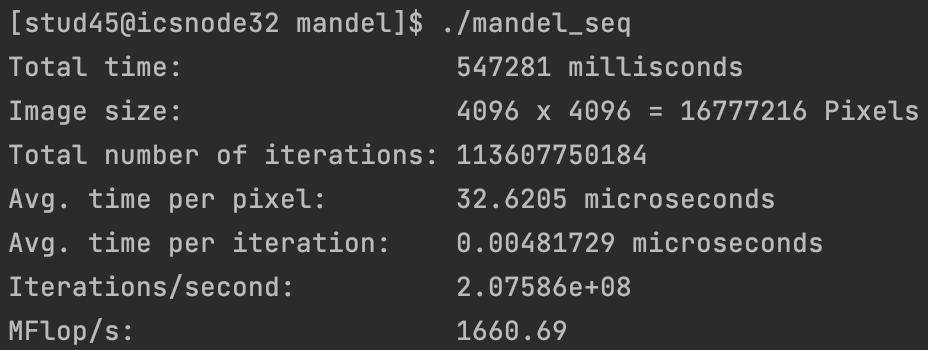
\includegraphics[width=0.7\linewidth]{bench_seq.png}
\end{center}
And this is the outputted Mandelbrot set visualization:
\begin{center}

\includegraphics[width=0.7\linewidth]{mandel.png}
\end{center}
I wanted to directly calculate the module of z by using sqrt(x2 + y2), but it didn't work, so instead of $|z| < 2$ I just used (x2 + y2) $<$ 4.
\newline
\newline
The OpenMP implementation wasn't that straightforward: after creating a new C file, mandel\_omp.c, while copying the contents of mandel\_seq.c, and adding it to the makefile with the -fopenmp option, I had a bit of trouble actually implementing the parallelization.
\newline
By defining all the variables as private, each thread should have no problem working on its own set of iterations, since they should all have their "sector" of the image to work in, but I always get an image with repeating horizontal patterns.
\begin{center}

\includegraphics[width=0.7\linewidth]{mandelomp.png}
\end{center}

\section{Bug hunt [15 points]}

\textbf{bug1.c}: The private variable tid was outside the for loop.
\newline
\textbf{bug2.c}: The ending thread tid didn't get printed correctly, it had to be declared private so that each thread would save its own tid.
\newline
\textbf{bug3.c}: The barrier just before the "Thread tid done and synchronized." printf command created the runtime error, since it is outside the critical section. My guess is that the various threads would all try to access the variable tid at the same time, but since there is a barrier, they caused a deadlock.
\newline
\textbf{bug4.c}: The stack size limit is too small and we are not allowed to increase it. A 2D array size NxN with N = 1048 is too much: changing N to 1023 sometimes gives segmentation fault and sometimes not, but 1022 seems to always work.
\newline
\textbf{bug5.c}: The locks' order resulted in a deadlock: opening two locks one after the other can stall the whole program if two or more threads try to access the same data and don't release the locks. Opening a lock on an array and closing it right after the needed operations are finished fixed the error.

\section{Parallel histogram calculation using OpenMP [15 points]}

The sequential implementation calculated the histogram in approximately 0.829 sec.
\newline
The parallel version showed the same result when using 1 thread, and then halved the time when using 2. Increasing the number of threads by one each time showed a logarithmic increase in performance up until 10 threads:
\newline
\newline
Threads = 1 | 0.829199 sec
\newline
Threads = 2 | 0.43775 sec
\newline
Threads = 3 | 0.291564 sec
\newline
Threads = 4 | 0.220706 sec
\newline
Threads = 5 | 0.175312 sec
\newline
Threads = 6 | 0.14716 sec
\newline
Threads = 7 | 0.125883 sec
\newline
Threads = 8 | 0.110019 sec
\newline
Threads = 9 | 0.0991479 sec
\newline
Threads = 10 | 0.0903315 sec
\newline
\newline
After 10, the performance seemed to worsen in the same logarithmic trend at first, but then it formed a plateau where the time fluctuates between 0.09 and 0.11 sec.
\newline
\newline
Threads = 11 | 0.100181 sec
\newline
Threads = 12 | 0.108046 sec
\newline
Threads = 13 | 0.110236 sec
\newline
Threads = 14 | 0.103181 sec
\newline
Threads = 15 | 0.104262 sec
\newline
Threads = 16 | 0.0935134 sec
\newline
Threads = 17 | 0.102403 sec
\newline
Threads = 18 | 0.0959442 sec
\newline
Threads = 19 | 0.118875 sec
\newline
Threads = 20 | 0.0922342 sec
\newline
\newline
The plateau seemed to remain flat even with 100+ threads, so it looks like 10 is the perfect number, at least for this specific program. I'm guessing that to see better results with more threads, the calculations need to be harder to compute.

\section{Parallel loop dependencies with OpenMP [15 points]}

Sequential RunTime :  6.717070 seconds
\newline
Final Result Sn    :  485165097.62511122
\newline
Result $||opt||^2_2$ :  5884629305179574.000000
\newline
\newline
These are the results of the sequential version of the given exercise. The goal is to parallelize Sn's calculation to reduce the runtime, while also keeping $opt^2_2$'s result the same.
\newline
Using the \textit{reduction} clause with 10 threads on Sn greatly increases performance (0.709001 sec, almost 10 times faster), but $opt^2_2$ is now equal to 13.399537: this is because each thread is working on their own version of opt, but only the last one gets saved, and since they are dividing the work between them, opt[N] is only a fraction of what it should be. Using only 1 thread fixes that problem, but now the runtime is equal to the sequential implementation.
\newline
\newline
Using the firstprivate and lastprivate clauses can help with that: the idea is to make sure than Sn gets multiplied the correct n number of times no matter what thread works on it. First, we declare Sn both firstprivate and lastprivate: this ensures that each thread saves the variable back into global memory after it finishes, and that it gets used by the next thread that starts working. Then, we have to declare a variable, in this case called exponent, that will be used to keep track of how many times Sn should be multiplied.
If exponent is equal to n, the calculations are done like in the sequential implementation and exponent becomes equal to n+1 (so basically just increments by 1); if exponent is not equal to n, Sn additionally gets multiplied by up\textsuperscript{n-exponent}.  Doing this makes sure that both Sn and opt are now correct, albeit with very slightly different values than those in the sequential implementation, and the runtime is greatly reduced:
\newline
\newline
Parallel RunTime   :  0.398345 seconds
\newline
Final Result Sn    :  485165097.62503791
\newline
Result $||opt||^2_2$ :  5884629305177205.000000
\newline
\newline
The best times were had while using 20 threads.


\section{Task:  Quality of the Report [15 Points]}





\end{document}
